\subsection{Soluzioni ideali}
Supponiamo di avere due liquidi in soluzione, ad esempio alcol etilico e acqua. Diciamo che questa soluzione è \textit{ideale} se per i due liquidi, i quali devono essere totalmente miscibili, cioè A si scioglie totalmente in B o viceversa B si scioglie totalmente in A qualunque siano le proporzioni, il $\Delta$H di mescolamento è pari a zero.

Di norma il $\Delta$H è diverso da zero, ma spesso si lavora con soluzioni diluite e pertanto le condizioni in cui lavoriamo sono prossime all'idealità.

\vspace{0.2cm}I liquidi hanno la caratteristica di evaporare, ed è evidente che se evaporano avremo particelle di A e di B in fase vapore. Nelle condizioni di idealità dei gas sappiamo che ogni specie gassosa si comporta come se fosse l'unica presente nel contenitore, pertanto se sia il vapore di A che quello di B viene assimilato ad un gas ideale ed ognuno dei due si comporterà come se fosse l'unico presente. Quindi la pressione totale potrà essere calcolata come somma delle pressioni parziali dei componenti A e B:
$$P=P_A + P_B \quad \text{(Legge di Dalton)}$$
Ovviamente stiamo immaginando di trovarci ad una data temperatura, cioè fissiamo una temperatura alla quale troviamo una certa pressione/tensione di vapore dovuta al componente A e un'altra dovuta al componente B e la cui somma dà la pressione totale.

Se non avessimo questa soluzione, quale sarebbe la tensione di vapore di ognuna delle due specie pure? 

Innanzitutto indichiamo con $P^0_A$ e $P^0_B$ le tensioni di vapore di ognuno dei due liquidi puri alla temperatura $T$ alla quale stiamo lavorando. Quindi, fissata la temperatura, il componente A eserciterà la pressione $P^0_A$ se puro, mentre se è in miscela eserciterà la pressione $P_A$. Analogamente per il componente B.

Qual è la relazione tra $P^0_A$ e $P_A$?

La loro relazione è data dalle \textit{legge di Raoult}, la quale dice che la pressione parziale di un componente in soluzione ideale ad una data temperatura $T$ è pari alla tensione di vapore di quel componente puro alla stessa temperatura, moltiplicata per la sua frazione molare:
$$P_A=\rchi_A P^0_A
\quad,\quad P_B=\rchi_B P^0_B \qquad \text{Legge di Raoult}$$
Poichè la frazione molare di ogni componente è sempre inferiore a 1, si ha sempre $P_A < P^0_A$. Quindi si ha un abbassamento delle tensioni di vapore delle singole specie quando le mettiamo in soluzione.

Inoltre, al variare della composizione della miscela variano anche le frazioni molari e di conseguenza varieranno $P_A$ e $P_B$, ma in generale la pressione sarà sempre data dalla legge di Dalton:
$$P=\rchi_A P^0_A + \rchi_B P^0_B$$
Ovviamente per calcolarla dovremo fissare temperatura e composizione.

Va da notare che $\rchi_A$ e $\rchi_B$ sono le frazioni molari in soluzione, mentre con questo metodo abbiamo calcolato la pressione del vapore. Allora quale sarà la composizione del vapore alla stessa temperatura?

Intuitivamente possiamo dire che nella fase vapore avremo più abbondanza del componente più volatile\footnote{La volatilità è la tendenza delle sostanze liquide o solide a passare allo stato di vapore.}. Dobbiamo però quantificare.

Abbiamo supposto che la soluzione sia ideale, per cui i vapori si comporteranno idealmente, cioè come se ognuno di loro fosse l'unico ad occupare l'intero volume a disposizione.

Se trattiamo i vapori come gas ideali avremo

$$P_AV=n_ART
\quad,\quad
P_BV=n_BRT$$

Sommiamo le espressioni:

$$(P_A + P_B)V= (n_A + n_B)RT$$

Dalla legge di Dalton sappiamo che la somma delle pressioni parziali è pari alla pressione totale:

$$P=P_A + P_B \implies PV=(n_A + n_B)RT$$

Questa espressione ci permette di avere informazioni sulla fase vapore. Tuttavia adesso $n_A$ e $n_B$ non sono le moli in soluzione, ma le moli in fase vapore.

Dividiamo entrambe le espressioni per quest'ultima:

$$\frac{P_AV}{PV}= \frac{n_ART}{(n_A + n_B)RT}
\implies
\frac{P_A}{P} = \frac{n_A}{n_A + n_B}\equiv \rchi '_A
\implies
P_A=P \cdot \rchi '_A$$

Questa sarà la frazione molare di A in fase vapore. Un risultato analogo si ottiene per B: $P_B=P \cdot \rchi '_B$.

Esplicitando P si otterrà
$$\rchi '_A=\frac{P_A}{P}=
\frac{P_A}{\rchi_A P_A^0 + \rchi_B P_B^0}=
\frac{\rchi_A P_A^0}{\rchi_A P_A^0 + \rchi_B P_B^0}$$

$$\rchi '_B=\frac{P_B}{P}=
\frac{P_B}{\rchi_A P_A^0 + \rchi_B P_B^0}=
\frac{\rchi_B P_B^0}{\rchi_A P_A^0 + \rchi_B P_B^0}$$
Questi calcoli sono necessari in quanto di norma il vapore non avrà la stessa composizione della soluzione a meno che vengano usati due liquidi con la stessa volatilità, cioè con la stessa temperatura di ebollizione.

A questo punto riscriviamo le equazioni delle frazioni molari in fase vapore dividendo numeratore e denominatore rispettivamente per $P_A^0$ e $P_B^0$:
$$\rchi'_A=\frac{\rchi_A}{\rchi_A + \rchi_B\frac{P^0_B}{P^0_A}}
\quad,\quad
\rchi'_B=\frac{\rchi_B}{\rchi_A\frac{P^0_A}{P^0_B} + \rchi_B}$$
In questo modo abbiamo delle relazioni tra frazioni molari in fase vapore e frazioni molari in soluzione.

Per definizione la somma delle frazioni molari è pari a 1, cioè $\rchi_A + \rchi_B =1$. Si avranno allora tre casi:
\begin{itemize}
    \item $P_A^0=P_B^0$, cioè i due liquidi hanno la stessa tensione di vapore. Allora dalle espressioni precedenti avremo che $\rchi_A'=\rchi_A$ e $\rchi_B'=\rchi_B$, ossia la composizione del vapore è identica a quella della soluzione, in quanto stessa tensione di vapore implica stessa volatilità;
    \item $P_B^0>P_A^0$, cioè a parità di temperatura la tensione di vapore del liquido puro B è maggiore di quella del liquido puro A. Ne segue che B è più volatile e in fase vapore ne troviamo di più.
    
    In questo caso $\frac{P_B^0}{P_A^0}>1$, per cui $\Big[\rchi_A + \rchi_B\frac{P_B^0}{P_A^0}\Big]>1$ e quindi $\rchi_A' < \rchi_A$ e in modo analogo $\rchi_B' > \rchi_B$, cioè essendo B più volatile la composizione del vapore sarà più ricca in B e meno in A.
    \item  $P_A^0>P_B^0$, cioè a parità di temperatura A è più volatile, quindi stavolta il vapore sarà più ricco nel componente A nonostante la composizione della soluzione.
    
    Si avrà quindi $\rchi_A' > \rchi_A$ e $\rchi_B' < \rchi_B$,
\end{itemize}

Consideriamo adesso un grafico in cui, fissata la temperatura, abbiamo in ascissa la frazione molare e nelle ordinate la tensione di vapore:

\begin{minipage}{0.4\textwidth}
    \begin{figure}[H]
        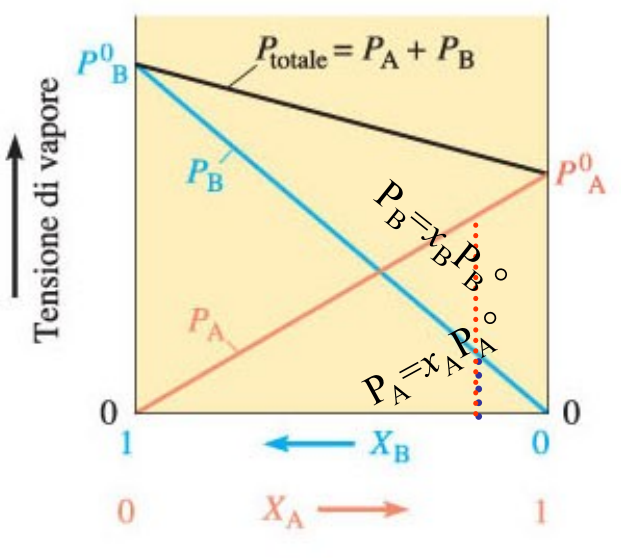
\includegraphics[width=6cm]{immagini/tensione_di_vapore_sol_ideale.png}
    \end{figure}
\end{minipage}
\begin{minipage}{0.6\textwidth}
    Nell'origine avremo il 100\% di B mentre A è assente (0\%). Man mano che ci spostiamo lungo le ascisse aumenta A, fino ad arrivare al punto opposto in cui abbiamo lo 0\% di B e il 100\% di A. Ovviamente la frazione molare è data in numeri, quindi negli estremi una vale 1 e l'altra vale 0.

    Per quanto riguarda le ordinate, nel punto in cui si ha il 100\% di B avremo la tensione di vapore di B puro, cioè $P^0_B$, mentre nel punto opposto in cui abbiamo solo A avremo la tensione di vapore del liquido A puro, cioè $P^0_A$.
\end{minipage}

Le due linee oblique rosse e blu rappresentano tutte le possibili tensioni di vapore (pressioni parziali) di ognuno dei componenti al variare della composizione della miscela. La linea nera rappresenta la somma di tutte le possibili pressioni totali, ottenute sommando le ordinate.

Tale grafico è valido solo se la soluzione è ideale, cioè se il $\Delta$H di mescolamento è pari a zero, ossia è valido se siamo nel campo di validità della legge di Raoult.

\vspace{0.2cm}E se invece la soluzione non è ideale, cioè se mostra un $\Delta$H di mescolamento diverso da zero?

Le soluzioni ideali sono rare, per cui di norma si hanno comportamenti che deviano dalla legge di Raoult.

L'obiettivo è quello di conoscere la termodinamica di queste soluzioni per poterla sfruttare per separare la soluzione nei suoi componenti. Ci è quindi utile conoscere la composizione del vapore per poterlo trattare col fine di arrivare ad una composizione diversa (separandolo dal liquido e condensandolo). Ad esempio in una soluzione di acqua e alcol non è possibile separare per distillazione acqua e alcol: si arriva ad un certo punto e poi non si riesce più. Dobbiamo capire perché.

\subsection{Processo di solubilizzazione endotermico}

Immaginiamo che il $\Delta$H sia diverso da zero, ad esempio maggiore di zero. Ciò significa che il sistema sta assorbendo calore, ossia per potere sciogliere A e B dobbiamo riscaldare, cioè dobbiamo fornire energia altrimenti la soluzione non si forma. Ciò capita tutte le volte in cui le interazioni che verranno a formarsi tra A e B sono più deboli di quelle che esistono nei liquidi puri, ovvero le interazioni A-A e B-B (per formare una soluzione si devono separare le particelle di soluto e quelle di solvente. Separare significa rompere le interazioni che si esercitano tra i componenti puri, cioè tra le loro molecole). 

\vspace{-0.1cm}\begin{minipage}{0.4\textwidth}
    \begin{figure}[H]
        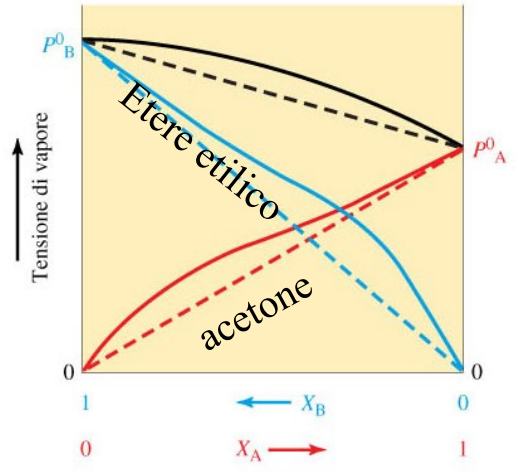
\includegraphics[width=6cm]{immagini/tensione_di_vapore_sol_endotermica.png}
    \end{figure}
\end{minipage}
\begin{minipage}{0.6\textwidth}

\vspace{0.4cm}In questo grafico le linee tratteggiate indicano il comportamento ideale, quelle continue descrivono il comportamento sperimentale, ottenuto misurando la tensione di vapore con varie composizioni.

Siccome le interazioni tra A e B sono più deboli, è chiaro che andranno più facilmente in fase vapore a parità di temperatura. Ne segue che per entrambe le specie avremo tensioni di vapore più alte di quelle ideali e di conseguenza sarà maggiore anche la tensione di vapore della soluzione rispetto a quella prevista dalla legge di Raoult.
\end{minipage}

\vspace{0.3cm}Il grafico riporta l'esempio di etere etilico CH$_3$-CH$_2$-O-CH$_2$-CH$_3$ e acetone CH$_3$-CO-CH$_3$. Fra le molecole di acetone si esercita una certa interazione e analogamente succede tra le molecole di etere etilico. Tra l'altro queste sono minori delle prime, infatti la tensione di vapore dell'etere etilico puro è maggiore di quella dell'acetone puro.

Nella soluzione le molecole di etere etilico interagiscono con le molecole di acetone, e la soluzione mostra una tensione di vapore maggiore di quella ideale perché queste interazioni sono più deboli di quelle osservate nei componenti puri.

Dal grafico possiamo evincere inoltre le temperature di ebollizione perché se a parità di temperatura la tensione di vapore di B è maggiore di quella di A vorrà dire che il punto di ebollizione di B è più basso di quello di A, cioè ad una data temperatura l'etere etilico è più volatile dell'acetone, per cui contribuirà di più alla tensione di vapore totale.

\subsection{Processo di solubilizzazione esotermico}

Consideriamo ora il caso opposto, cioè una soluzione non ideale con $\Delta$H$<$0. Ciò significa che il sistema libera energia, cioè la cede all'ambiente. In questi casi si ha un processo di solubilizzazione esotermico, il quale avviene nel caso opposto al precedente, cioè quando tra A e B si esercitano interazioni molto più forti di quelle che si esercitavano tra le molecole di A e tra le molecole di B nei liquidi puri. In conseguenza a ciò si avrà meno vapore e quindi meno tensione di vapore, ossia il sistema è meno volatile perché tra A e B si sono instaurate interazioni forti che devono essere rotte per far evaporare la soluzione.

\vspace{-0.2cm}\begin{minipage}{0.4\textwidth}
    \begin{figure}[H]
        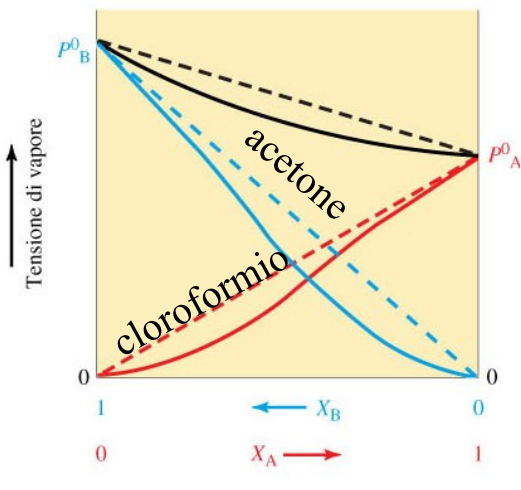
\includegraphics[width=6cm]{immagini/tensione_di_vapore_sol_esotermica.png}
    \end{figure}
\end{minipage}
\begin{minipage}{0.6\textwidth}
    Consideriamo una soluzione formata da acetone CH$_3$-CO-CH$_3$ e cloroformio CHCl$_3$.

    Le tensione di vapore del cloroformio puro è minore di quella dell'acetone puro. Ciò significa che a parità di temperatura la specie B è più volatile. Inoltre sperimentalmente si osserva che entrambi i componenti hanno tensioni di vapore minori di quelle previste dall'idealità, e quindi anche la soluzione avrà un comportamento che mostra un abbassamento della tensione di vapore.
\end{minipage}
\E inoltre conveniente, essendo una reazione che sprigiona calore, allontanare quest'ultimo, in quanto raffreddando il processo di dissoluzione viene facilitato.

La reazione sarà

$$\ce{A + B ->} \text{soluzione + calore}$$

Il motivo è che il calore può essere sia un reagente che un prodotto. Nel caso in cui sia un prodotto, nel momento in cui lo allontaniamo la reazione ne produrrà altro, ma questo comporterà la creazione di altra soluzione. In altre parole, allontanare i prodotti significa spostare verso destra quella reazione.